\begin{figure}[tb]
	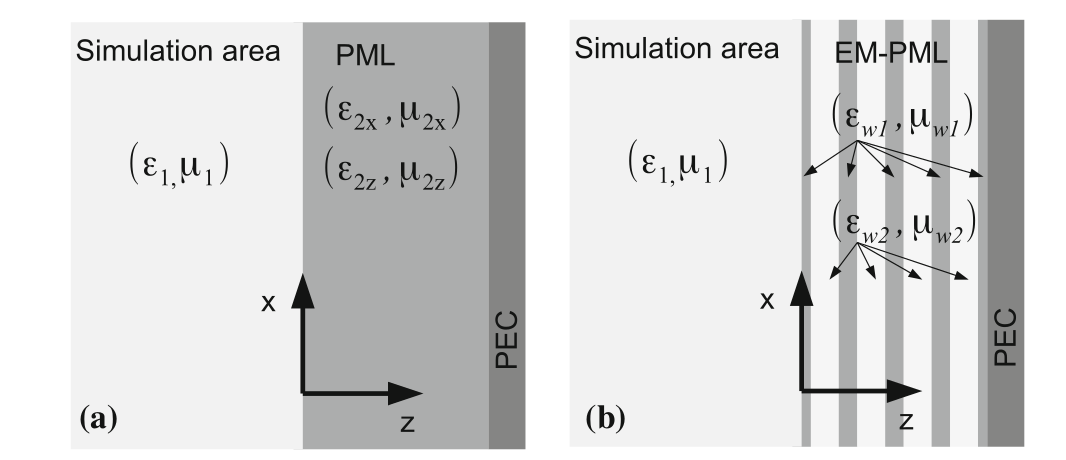
\includegraphics[width=\textwidth]{images/pml/oqe_schemat.png}
	\caption{Schematyczne przedstawienie analizowanej struktury warstwowej i przybliżanego za pomocą modelu ośrodka efektywnego ośrodka PML}
	\label{fig:pml-multilay-schem}
\end{figure}

Porównując ogólną postać PML podaną w równaniu (\ref{eq:general-pml-form}) z modelem ośrodka efektywnego przedstawionym w podrozdziale \ref{subart:effmedium} można zaproponować przybliżenie ośrodka typu PML za pomocą struktury warstwowej o odpowiednich właściwościach efektywnych. W szczególności, dla uproszczenia analizy, skupimy się na polaryzacji TM, dla której istotnymi składowymi tensorów opisujących własności materiałowe są:~$\varepsilon_x$~,$\mu_y$~i $\varepsilon_z$. Ze względu na ograniczenia używanego modelu ośrodka efektywnego, zgodnie ze schematem na rysunku \ref{fig:pml-multilay-schem} $\varepsilon_x=\varepsilon_y$, oraz $\mu_x=\mu_y$. Ponownie odwołując się do granicy między ośrodkami na rysunku \ref{fig:pml-multilay-schem}a warunki dla których wielowarstwa złożona z materiałów $w1$ i $w2$ schematycznie przedstawiona na rysunku \ref{fig:pml-multilay-schem}b będzie efektywnie spełniać rolę PML pod warunkiem spełnienia następujących równości:
\begin{equation}
	f\cdot \varepsilon_{w1} + (1-f)\cdot \varepsilon_{w2} = s \cdot \varepsilon_1,
	\label{eq:oqe4}
\end{equation}

\begin{equation}
	[f\cdot \varepsilon_{w1}^{-1}+(1-f)\varepsilon_{w2}^{-1}]^{-1}=s^{-1}\cdot \varepsilon_1,
	\label{eq:oqe5}
\end{equation}

\begin{equation}
	f\cdot \mu_{w1} + (1-f)\cdot \mu_{w2} = s \cdot \mu_1,
	\label{eq:oqe6}
\end{equation}
gdzie przez $f$ oznaczony został współczynnik wypełnienia, równy ułamkowi przestrzeni wielowarstwy zajmowanemu przez materiał $w1$. Odpowiednie warunki dla polaryzacji TE to:
\begin{equation}
	\varepsilon_{w1}=\rho \frac{\varepsilon_1 \cdot s}{f\cdot \rho + (1 -f) },
	\label{eq:te-eps1}
\end{equation}

\begin{equation}
	\varepsilon_{w2}=\frac{\varepsilon_1 \cdot s}{f\cdot \rho + (1-f)},
	\label{eq:te-eps2}
\end{equation}
gdzie
\begin{equation}
	\rho = 1+\frac{s^2-1 \pm \sqrt{(s^2-1)(s^2-(2f-1)^2)}}{2f(1-f)}.
	\label{eq:te-rho}
\end{equation}

\begin{figure}[tb]
	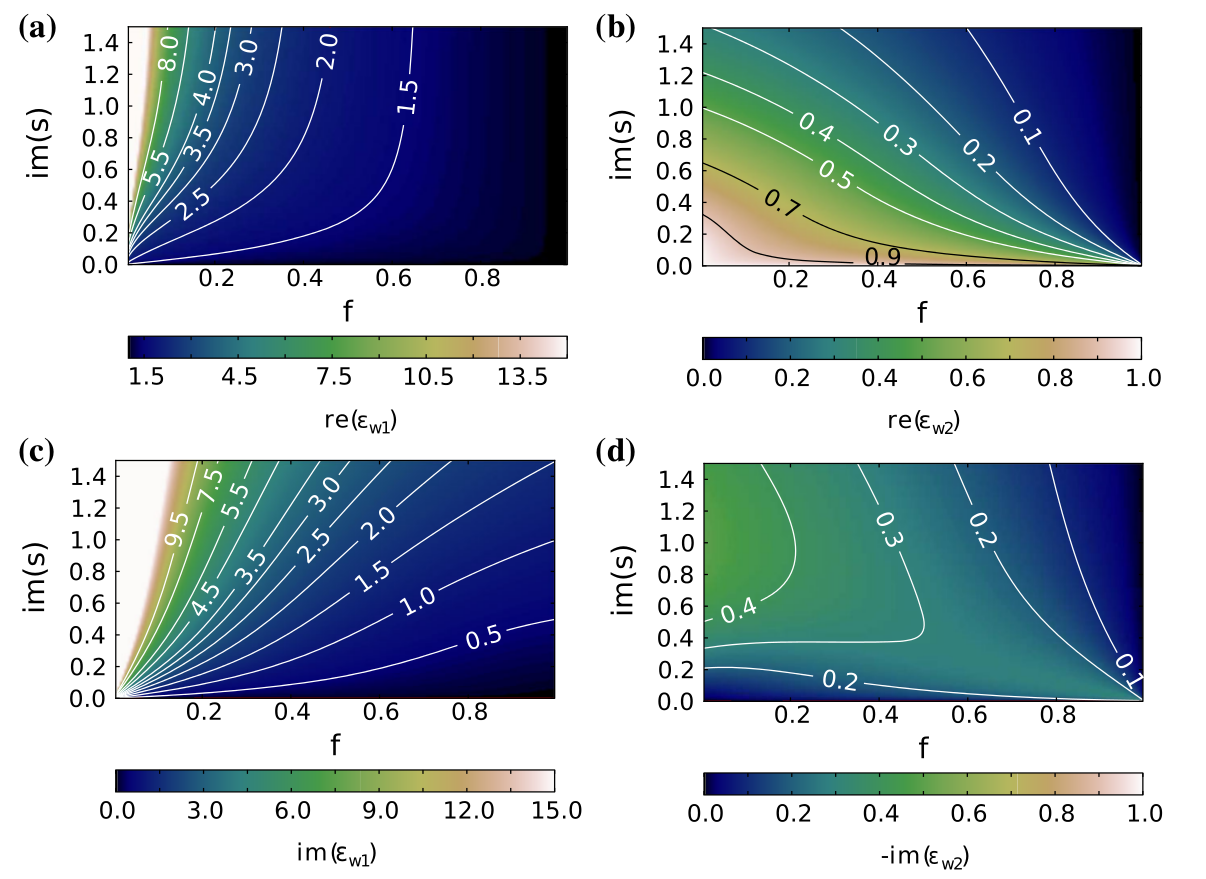
\includegraphics[width=\textwidth]{images/pml/oqe_materials.png}
	\caption{Zależność przenikalności elektrycznej materiałów tworzących UPML (w lewej kolumnie $\varepsilon_{w1}$, w prawej $\varepsilon_{w2}$) w funkcji współczynnika wypełnienia i urojonej części parametru $s$ (założono, że $\textrm{Re}(s)$=1. Górny wiersz na wykresach (a) i (b) prezentuje zależności części rzeczywistych, dolny na wykresach (c) i (d) części urojonych przenikalności elektrycznych. Ujemne wartości $\varepsilon$ na wykresach (c) i (d) odpowiadają materiałom ze wzmocnieniem optycznym. }
	\label{fig:upml-eps-s-f}
\end{figure}

Wykresy na rysunku \ref{fig:upml-eps-s-f} prezentują wyniki obliczonych zgodnie z (\ref{eq:te-eps1}) i (\ref{eq:te-eps2}) wartości $\varepsilon_{w1}$ i $\varepsilon_{w2}$ jako funkcje współczynnika wypełnienia $f$ i parametru $s$, dla którego przyjęto $s=1+\alpha i$. Używamy rozwiązań dla (\ref{eq:te-rho}) z $|\rho|>1$. Podobne wyrażenia jak (\ref{eq:oqe4}) i (\ref{eq:oqe5}) można wypisać i rozwiązać dla $\mu_{w1}$ i $\mu_{s2}$. W przypadku gdy $\varepsilon_1=\mu_1$ otrzymujemy $\varepsilon_{w1}=\mu_{w1}$ i $\varepsilon_{w2}=\mu_{w2}$. Należy podkreślić, że dla każdej pary $f$ i $s$ przedstawionej na wykresach \ref{fig:upml-eps-s-f} uzyskujemy metamateriał, który w omawianym przybliżeniu będzie spełniał funkcje UPML, dla każdej pary $f$ i $s$ potrzebujemy jednak wybrać inne materiały $w1$ i $w2$.

W kolejnym kroku możemy obliczyć natężeniowy współczynnik odbicia od strukutury zaprezentowanej na rysunuku \ref{fig:pml-multilay-schem}b dla $f=0.6$, oraz $\textrm{Im}(s)=$0.5 lub $\textrm{Im}(s)=$5. Zależność współczynnika odbicia od kąta padania, oraz grubości komórki elementarnej wielowarstwy przedstawia wykres na rysunku \ref{fig:oqe3}. Ze względu na umieszczenie idealnego przewodnika za wielowarstwą współczynnik odbicia łączy w sobie część odbijaną od wielowarstwy, jak i transmitowaną przez wielowarstwę i odbijaną od zwierciadła z PEC. Analizując wykres \ref{fig:oqe3} możemy zauważyć, że wraz ze wzrostem $\frac{a}{\lambda}$ zmniejsza się współczynnik odbicia fal propagujących się, którym odpowiada część wykresu dla którego na osi odciętych wartości spełniają nierówność
\[ 
\frac{k_x}{k_0}<1.
\] Wynika to ze zwiększania grubości warstwy pochłaniającej, więc jest przede wszystkim związane ze zmniejszeniem transmisji przez wielowarstwę, a nie zmianą odbicia od pierwszej granicy warstw. W przypadku fal ewanescentnych $\frac{k_x}{k_0}>1$ obserwujemy wzrost współczynnika odbicia. Można to interpretować jako odbicie od pierwszej warstwy wynikające z niespełnienia warunków homogenizacji (przybliżenie ośrodka efektywnego zakłada $\frac{a}{\lambda} <<$ 1) przez strukturę. Dlatego wzrost jest większy dla większej części urojonej współczynnika $s$, skutkującej większą różnicą współczynników załamania na granicy pierwszej warstwy i powietrza.

\begin{figure}[tb]
	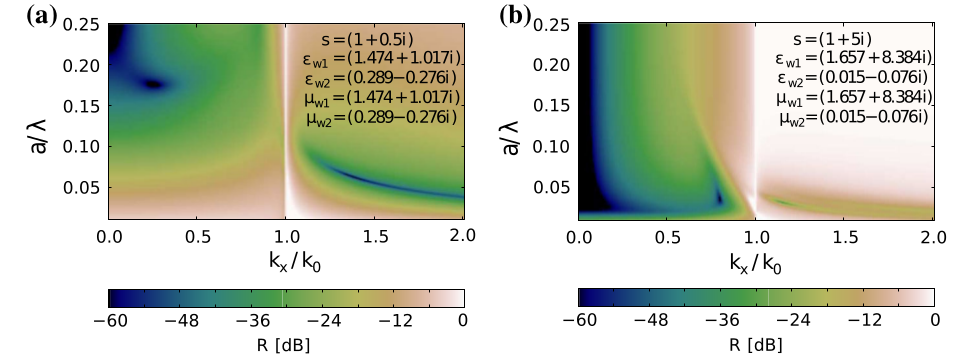
\includegraphics[width=\textwidth]{images/pml/fig3.png}
	\caption{Zależność natężeniowego współczynnika odbicia od kąta padania i okresu wielowarstwy dla struktury zgodniej ze schematem na rysunku \ref{fig:pml-multilay-schem}, dla $N=5$ par warstw, przy współczynniku wypełnienia $f=0.6$. Rysunek po lewej (a) przedstawia wyniki dla $s=1+0.5i$, wykres po prawej przedstawia wyniki dla $s=1+5i$.}
	\label{fig:oqe3}
\end{figure}

Przedstawione wyniki możliwe są do osiągnięcia za pomocą materiałów wykazujących szczególne własności elektryczne i magnetyczne. W szczególności obliczenia zakładały zespoloną przenikalność magnetyczną, oraz wzmocnienie optyczny. Dla $s=1+5i$ możliwe jest uzyskanie warstwy PML o całkowitej grubości $5\cdot a \approx \frac{\lambda}{20}$ wykazującej natężeniowy współczynnik odbicia ok -30dB dla szerokiego zakresu kątów padających fal płaskich.

W przypadku oświetlenia wielowarstwy za pomocą polaryzacji TM jeden ze współczynników przenikalności magnetycznej może zostać ustalony w sposób arbitralny. W szczególności możemy więc założyć $\mu_{w2}=1$, ponieważ większość materiałów spotykanych w przyrodzie charakteryzuje się taką wartością dla częstotliwości optycznych. Drugą przenikalność magnetyczną możemy wyznaczyć za pomocą wzoru \ref{eq:oqe6}. Część rzeczywista $\textrm{Re}(\mu_{w1})=1$, a zależność części urojonej $\textrm{Im}(\mu_{w1})$ od części urojonej współczynnika $s$, oraz współczynnika wypełnienia przedstawia wykres \ref{fig:im-mu1}. Na podstawie przywołanego wykresu możemy zauważyć, że wysoki współczynnik wypełnienia, oraz wykorzystanie niskiej części urojonej $s$ skutkują niskimi wartościami $\textrm{Im}(\mu_{w1})$. Jest to dla nas istotne ponieważ korzystając z realnych materiałów będziemy zmuszeni przybliżyć tę wartość przez $0$.

\begin{SCfigure}
	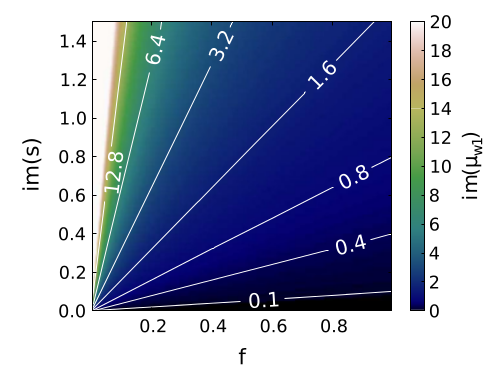
\includegraphics[width=0.6\textwidth]{images/pml/fig4.png}
	\caption{Zależność części urojonej przenikalności magnetycznej jednego z materiałów $\mu_{w1}$, od części urojonej współczynnika $s$ i współczynnika wypełnienia $f$ w przypadku gdy założono $\mu_{w2}=1$}
	\label{fig:im-mu1}
\end{SCfigure}


W przypadku przygotowania eksperymentu, a nie np. wykorzystaniu do konstrukcji PML w symulacjach  numerycznych, należy zaniedbać własności magnetyczne materiałów $\mu=1$, oraz zysk optyczny $\textrm{Im}(\varepsilon)\ge0$. Wyniki dla obu polaryzacji po zastosowaniu się do wymienionych przybliżeń przedstawiają wykresy na rysunku \ref{fig:pml-real-ref}. Zaproponowany absorber składa się z materiału stratnego, oraz warstw charakteryzujących się przenikalnością elektryczną mniejszą od 1. Przedstawione wyniki obliczeń wskazują, że w wyniku poczynionych założeń efektywność pracy wielowarstwy jako struktury PML znacznie różni się w zależności od polaryzacji. W przeciwieństwie do obliczeń dla wielowarstw odpowiadających PML, narzucone warunki prowadzą do mniejszej wartości współczynnika odbicia dla polaryzacji TE. Wysokie współczynniki odbicia, uniemożliwiające zastosowanie wielowarstwy,  pojawiają się jednak jedynie dla kątów padania bliskich $90^{\circ}$, co jest charakterystyczne dla UPML.

\begin{figure}[tb]
	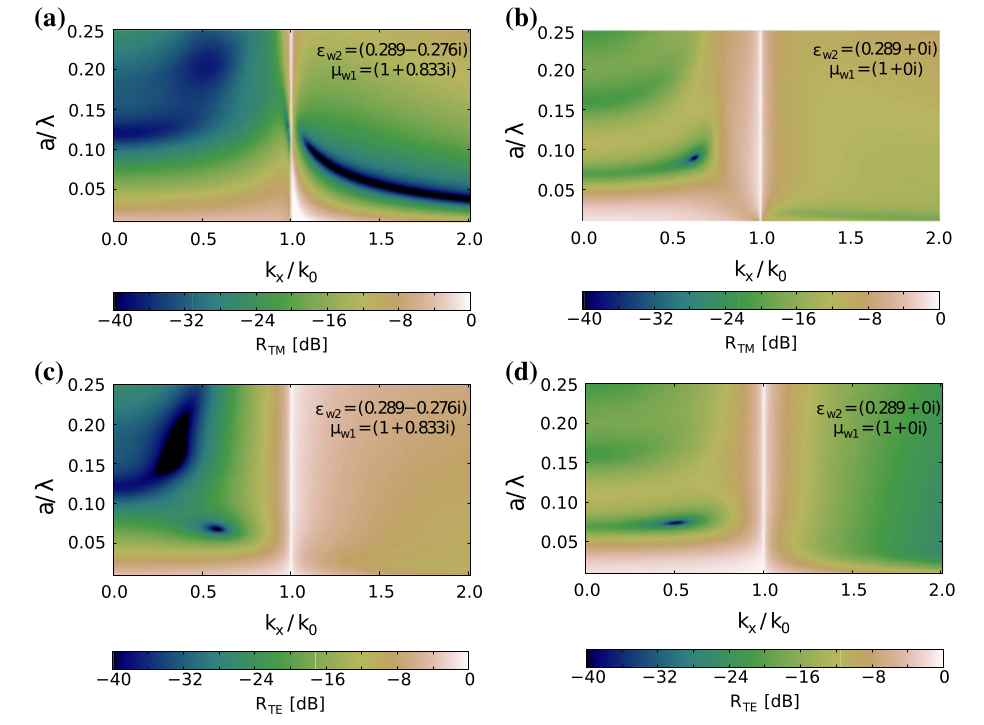
\includegraphics[width=\textwidth]{images/pml/fig5.png}
	\caption{Zależność natężeniowego współczynnika odbicia $R$, od kąta padania i grubości warstw dla wielowarstwy składającej się z $N=5$ okresów, dla $s=1+5i$ i $f=0.6$. Spełniając założenie, że $\mu_{w2}=1$ (a,c), oraz $\mu_{w1}=\mu_{w2}=1$, $\textrm{Im}(\varepsilon_1)\ge 0 $ i $\textrm{Im}(\varepsilon_2)\ge 0 $ (b,d). Wyniki dla polaryzacji TM (a,b) oraz TE (c,d). Przenikalność elektryczna $\varepsilon_{w1}=1.474+1.017i$.}
	\label{fig:pml-real-ref}
\end{figure}


Na podstawie przeprowadzonej dyskusji, można zaproponować prostą regułę jaką należy posługiwać się w celu doboru materiałów do budowy wielowarstwy efektywnie przypominającej UPML graniczący z powietrzem. Kluczowym elementem jest wykorzystanie materiału którego część rzeczywista przenikalności elektrycznej znajduje się w zakresie od 0 do 1. Przeprowadzone obliczenia wskazują również, że materiał ten powinien być możliwe bezstratny. Druga wykorzystywana substancja powinna posiadać część rzeczywistą przenikalności elektrycznej większą od 1, oraz wykazywać stratność. 

W ogólności w szerokich zakresach spektralnych większość materiałów charakteryzuje się $\textrm{Re}(\varepsilon) > 1$. Wyjątkami są zakresy długości fali w okolicach rezonansów dyspersyjnych (patrz. \ref{subart:lorenz-drude}). Możliwe jest również uzyskanie zaprojektowanych własności $\varepsilon$ w metamateriałach np. w strukturach funkcjonujących w literaturze angielskojęzycznej pod nazwą \textit{fishnet}~\cite{valentine2008three}. 

Przykładem pary materiałów, które możemy zastosować w realizacji UPML za pomocą wielowarstwy są $SiO_2$ i $NaCl$ dla długości fali w okolicach 8~$\mu$m. Przenikalności elektryczne zaproponowanych materiałów przedstawiają wykresy na rysunku \ref{fig:nacl-sio2-mat}. Rolę materiału o przenikalności elektrycznej $\varepsilon \in (0,1)$, spełnia w tym obszarze $SiO_2$, ponieważ dla długości fali $9.5$~$\mu$m występuje dla tego materiału rezonans, również wartość efektywna części urojonej wielowarstwy wynika głównie z własności $SiO_2$. 

\begin{figure}[tb]
	\begin{subfigure}{0.45\textwidth}
		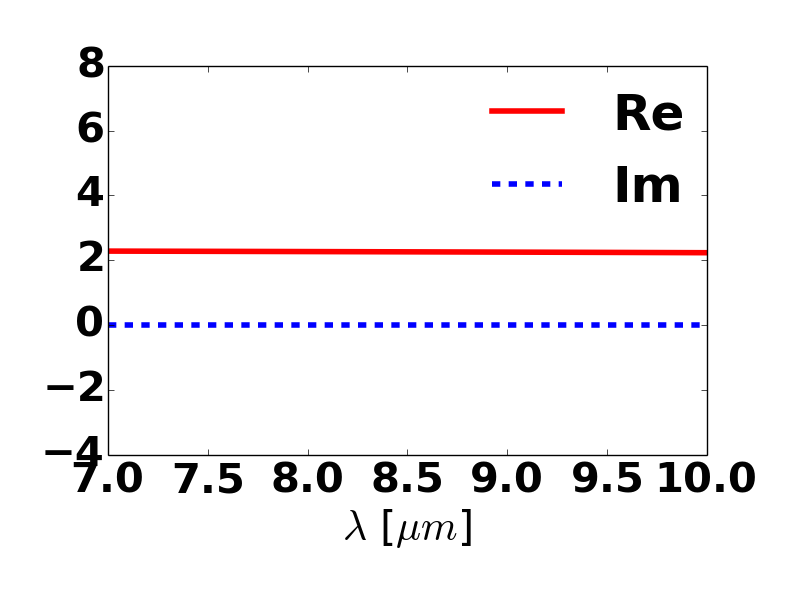
\includegraphics[width=\textwidth]{images/pml/nacl.png}
		\caption{}
	\end{subfigure}
	\begin{subfigure}{0.45\textwidth}
		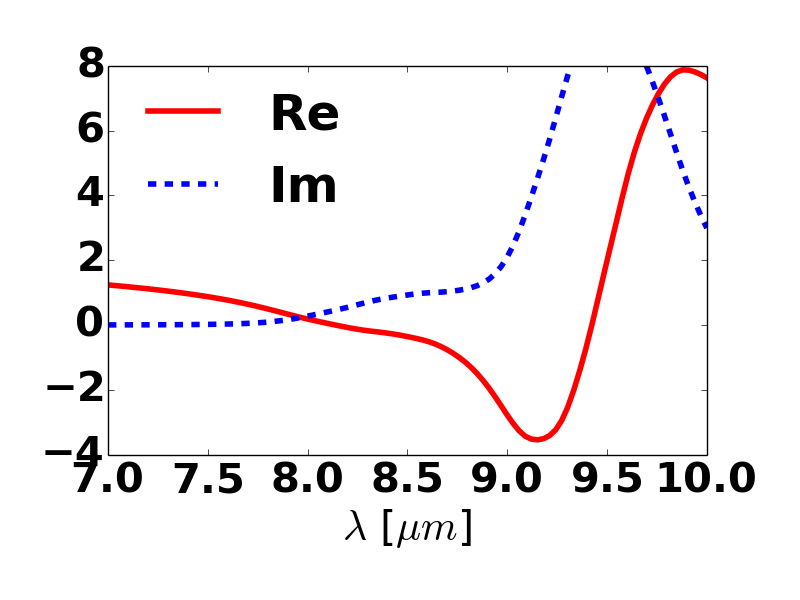
\includegraphics[width=\textwidth]{images/pml/sio2.png}	
		\caption{}
	\end{subfigure}
	\caption{Wartości przenikalności elektrycznej w zakresie od 7 do 10~$\mu$m dla (a) $NaCl$~\cite{li1976refractive}, (b) $SiO_2$~\cite{Kischkat:12}}
	\label{fig:nacl-sio2-mat}
\end{figure}

Efektywne własności stosu złożonego z naprzemiennych warstw $NaCl$ i $SiO_2$ o współczynniku wypełnienia drugim materiałem $f=0.56$, dla których przyjęto zmierzone eksperymentalnie wartości $\varepsilon$ przedstawia wykres na rysunku \ref{fig:eff-pml-real}. Zgodnie z (\ref{eq:general-pml-form}) struktura warstwowa przypominająca PML powinna charakteryzować się $\frac{1}{\varepsilon_x}=\varepsilon_z$, dlatego na wykresie zaznaczono również wartość $\frac{1}{\varepsilon_x}$. Na podstawie wykresu \ref{fig:eff-pml-real}, wielowarstwa powinna więc charakteryzować się najniższym współczynnikiem odbicia dla długości fali z zakresu 8.0-8.2~$\mu$m. Wartości natężeniowych współczynników transmisji i odbicia w zależności od liczby par warstw $N$ oraz długości fali przedstawia wykres na rysunku \ref{fig:oqe-trans-refl}.

\begin{SCfigure}
	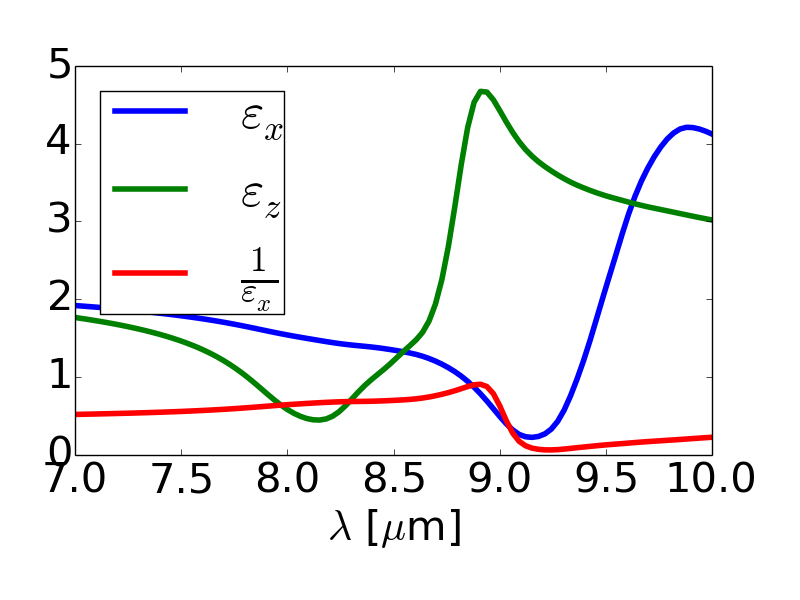
\includegraphics[width=0.6\textwidth]{images/pml/effepsilon-nacl-sio2.png}
	\caption{Współczynniki efektywne wielowarstwy zbudowanej z $SiO_2$ i $NaCl$, o współczynniku wypełnienia przez $SiO_2$ równym $f=0.56$.}
	\label{fig:eff-pml-real}
\end{SCfigure}

Bazując na zaprojektowanej wielowarstwie można zaproponować jej realizację w geometrii cylindrycznej. W tym przypadku jakość nieodbijającej warstwy absorpcyjnej możemy ocenić na podstawie symulacji, w których wewnątrz struktury typu \textit{core-shell} zamknięty zostanie walec z idealnego przewodnika. Rozkład gęstości energii pola E-M dla struktury typu core-shell odpowiadającą rozważanej wielowarstwie, oświetloną falą monochromatyczną dla polaryzacji TM~i~TE przedstawia rysunek \ref{fig:oqecoreshell}.

\begin{figure}[tb]
	\centering
	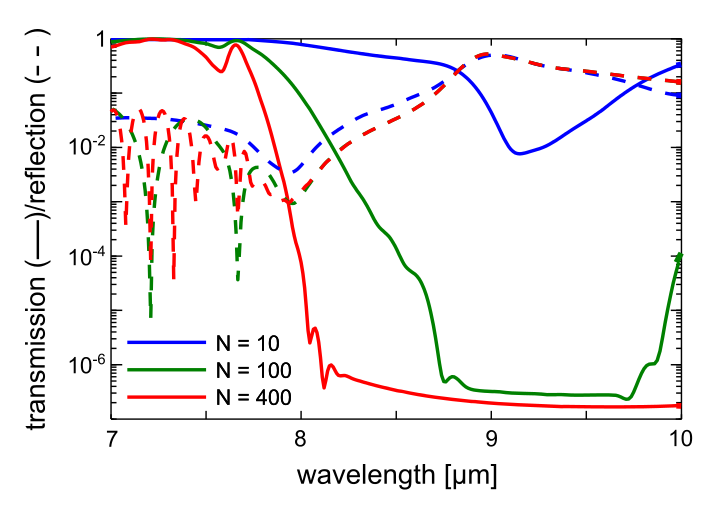
\includegraphics[width=0.6\textwidth]{images/pml/oqe_trans_refl.png}
	\caption{Współczynnik transmisji (linia ciągła) i odbicia (linia przerywana) dla wielowarstwy złożonej z $SiO_2$/$NaCl$ zaprojektowanej dla oświetlenia długością fali 8~$\mu$m, dla której współczynniki załamania $n_{\textrm{SiO}_2}=0.41+0.32i$, $n_{\textrm{NaCl}}=$~1.51. Współczynnik wypełnienia struktury przez $SiO_2$ wynosi $f=0.56$, $a=200nm$. Rozważone zostały stosy o liczbie par warstw $N=$~10,~100 i 400.}
	\label{fig:oqe-trans-refl}
\end{figure}

\begin{figure}[tb]
	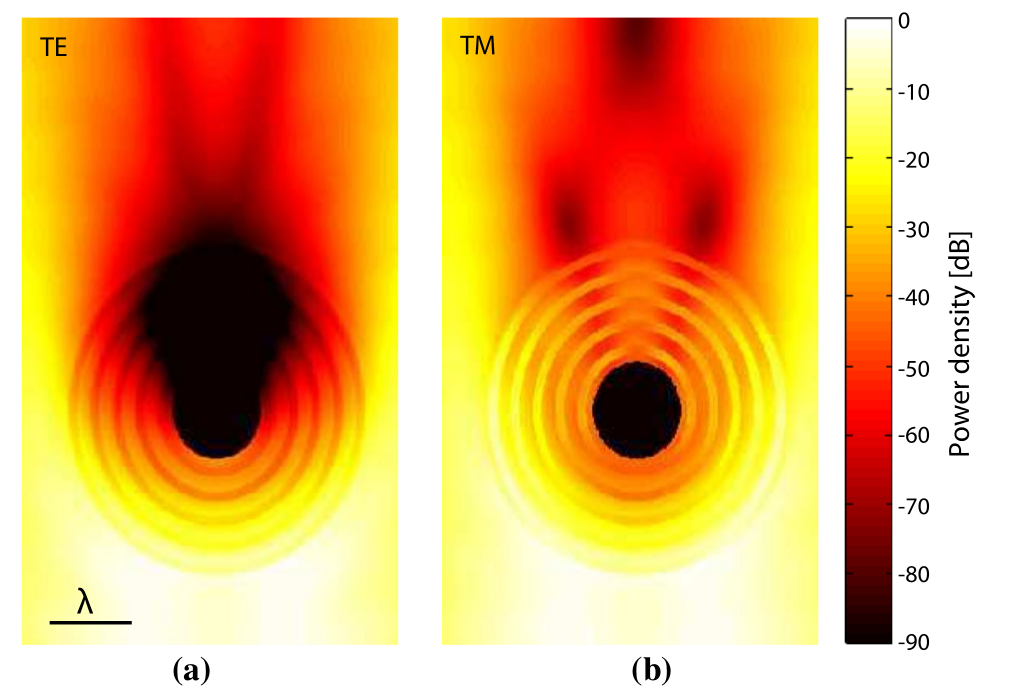
\includegraphics[width=\textwidth]{images/pml/oqe_coreshell.png}
	\caption{Wyniki symulacji we współrzędnych cylindrycznych dla polaryzacji (a) TE i (b) TM. Struktura typu core-shell oświetlona jest z dołu, na rysunku (a) zamieszczono wzorzec długości fali.}
	\label{fig:oqecoreshell}
\end{figure}


